%% ─────────────────────────────────────────────────────────────────────────
%%  Supplementary Material for:
%%  "Correction and Corruption Signals in Capability-Asymmetric
%%   Multi-Agent LLM Debate: A Bias-Theoretic Account"
%%  Author: Koushik Deb
%% ─────────────────────────────────────────────────────────────────────────
\documentclass[review,3p,authoryear]{elsarticle}

\usepackage{lineno}
\modulolinenumbers[5]

\journal{Cognitive Systems Research}

\usepackage{amsmath,amssymb}
\usepackage{graphicx}
\usepackage{booktabs}
\usepackage{multirow}
\usepackage{url}
\usepackage{hyperref}
\usepackage[british]{babel}
\usepackage{listings}
\usepackage{xcolor}

\bibliographystyle{elsarticle-harv}

%% ─────────────────────────────────────────────────────────────────────────
\begin{document}

\begin{frontmatter}

\title{Supplementary Material:\\
Correction and Corruption Signals in Capability-Asymmetric
Multi-Agent LLM Debate:
A Bias-Theoretic Account}

% \author[aff1]{Koushik Deb\corref{cor1}}
% \ead{k.deb@[institution].ac.uk}
% \cortext[cor1]{Corresponding author}

% \affiliation[aff1]{organization={[Department, Institution]},
%              addressline={[Address]},
%              city={[City]},
%              postcode={[Postcode]},
%              country={[Country]}}

\end{frontmatter}

\linenumbers

%% ═════════════════════════════════════════════════════════════════════════
\section*{S1. Full condition counts and trial-level statistics}
\label{ssec:counts}
%% ═════════════════════════════════════════════════════════════════════════

Table~\ref{stab:fullcounts} reports the number of trials per condition and
per focal model, the mean Round~0 accuracy, and the resulting Round~1
accuracy, confirming that no condition is under-powered.

\begin{table}[h]
\centering
\small
\caption{Full trial counts and per-round accuracy for all five conditions
and both focal models.
\label{stab:fullcounts}}
\begin{tabular}{@{}llrrrl@{}}
\toprule
Focal model & Cond. & Trials & R0 acc.\ (\%) & R1 acc.\ (\%) & $\Delta$ (pp) \\
\midrule
\multirow{5}{*}{\textit{DeepSeek-v4-flash}}
  & C1 & 1,500 & 76.2 & 76.2 & 0.0 \\
  & C2 & 1,500 & 76.2 & 78.7 & $+$2.5 \\
  & C3 & 1,500 & 76.2 & 78.3 & $+$2.1 \\
  & C4 & 1,500 & 76.2 & 84.1 & $+$7.9 \\
  & C5 & 1,500 & 76.2 & 82.5 & $+$6.3 \\
\midrule
\multirow{4}{*}{\textit{GPT-4o-mini}}
  & C1 & 250   & 64.8 & 64.8 & 0.0 \\
  & C2 & 250   & 64.8 & 66.8 & $+$2.0 \\
  & C3 & 250   & 64.8 & 60.8 & $-$4.0 \\
  & C4 & 250   & 64.8 & 65.2 & $+$0.4 \\
\bottomrule
\end{tabular}
\end{table}

%% ═════════════════════════════════════════════════════════════════════════
\section*{S2. McNemar test details}
\label{ssec:mcnemar}
%% ═════════════════════════════════════════════════════════════════════════

The McNemar test comparing C1 and C4 at the question level uses the
contingency matrix below, derived from 300 questions ($\times$~5
replications, majority-vote per question):

\[
\begin{pmatrix}
\text{C4 correct} & \text{C4 wrong} \\
218 & 33 \\
12  & 37
\end{pmatrix}
\quad
\begin{array}{l}
\text{(C1 correct, rows)} \\
\text{(C1 wrong, rows)}
\end{array}
\]

The off-diagonal counts are $b = 33$ (correct in C1, wrong in C4) and
$c = 12$ (wrong in C1, correct in C4).
McNemar's statistic gives $\chi^2 = (|b - c| - 1)^2 / (b + c) = 8.9$ on
1 degree of freedom, yielding $p = 0.0025$ (unadjusted) and
Bonferroni-adjusted $p = 0.017$ (five comparisons, $\alpha = 0.05$).
The test confirms a significant net regression of question-level correctness
under maximal dumb-peer exposure.

%% ═════════════════════════════════════════════════════════════════════════
\section*{S3. Calibration gate details}
\label{ssec:calibration}
%% ═════════════════════════════════════════════════════════════════════════

The calibration gate was run before the main experiment to determine whether
a confidence threshold of 60 could identify incorrect dumb-agent responses.
Across 1,500 dumb-agent trials (pooling both \textit{Llama~3.1~8B Instruct}
and \textit{Gemma~3~4B Instruct}), the proportion of incorrect responses
reporting confidence $\geq 60$ was 0.995 (95\% CI: [0.9909, 0.9983]).
The activation threshold for filtering to be informative was defined as
0.40 (i.e., if more than 40\% of incorrect responses were above the
threshold, the threshold would be inadequate).
Since $0.995 \gg 0.40$, the gate passed (confirmed filtering would fail)
and the experiment proceeded as designed, treating C5 as a deliberate
stress test of confidence-based filtering.

%% ═════════════════════════════════════════════════════════════════════════
\section*{S4. Prompt templates}
\label{ssec:prompts}
%% ═════════════════════════════════════════════════════════════════════════

The full system- and user-prompt strings are reproduced verbatim below.

% TODO\_FOR\_AUTHOR: choose path A or path B
% Path A (preferred): paste prompt strings here in verbatim blocks
% Path B (code release): replace this section with a sentence giving
% the public repository URL and commit hash.

\subsection*{Round-0 prompt (focal and smart agents)}
\begin{verbatim}
% TODO_FOR_AUTHOR: paste Round-0 prompt verbatim
\end{verbatim}

\subsection*{Round-1 prompt}
\begin{verbatim}
% TODO_FOR_AUTHOR: paste Round-1 prompt verbatim
\end{verbatim}

\subsection*{C5 filtered-peer preface}
\begin{verbatim}
% TODO_FOR_AUTHOR: paste C5 filter preface verbatim
\end{verbatim}

\paragraph{Judge cascade.}
When regular-expression and structured-parsing extraction both fail, a
three-judge cascade is invoked.
The primary judge is \textit{Gemini 2.5 Flash Lite} (via Google Generative
AI API); the fallback is \textit{Mistral Small}; the tertiary judge is
\textit{DeepSeek-v4-flash}.
Each judge is given the raw response text and the answer schema and
asked to extract the intended final answer.
Judge agreement was unanimous in 98.3\% of cascade invocations;
the remaining 1.7\% were resolved by majority vote among the three judges.

%% ═════════════════════════════════════════════════════════════════════════
\section*{S5. Persona categories and validation}
\label{ssec:personas}
%% ═════════════════════════════════════════════════════════════════════════

Four persona styles were used: analytical (precise, evidence-driven),
sceptical (doubt-expressing, question-challenging), diplomatic
(consensus-seeking, hedge-using), and assertive (confident, direct).
Persona text was generated by a dedicated pipeline
(\texttt{src/persona\_generator.py}) using \textit{DeepSeek-v4-flash}
as the generation model.
Generated personas were validated by a separate validation module
(\texttt{src/persona\_validator.py}) that checked for:
(a)~minimum length ($\geq$50 words);
(b)~absence of self-referential phrases (e.g.\ ``I am an AI'');
(c)~coherence score above a threshold set by an LLM judge.
Of 1,500 generated personas, 1,486 passed (retention rate 99.1\%).
The 14 failures were replaced by sampling from the validated pool.

%% ═════════════════════════════════════════════════════════════════════════
\section*{S6. Dataset composition}
\label{ssec:dataset}
%% ═════════════════════════════════════════════════════════════════════════

The 300-question pool consists of 250 questions sampled from
\textit{MMLU-Pro}~\citep{wang2024mmlupro} across ten subject categories
(25 questions per category) and 50 questions sampled from the
\textit{GSM8K}~\citep{cobbe2021training} test split.
Questions were stratified by difficulty tier (easy/medium/hard as
determined by MMLU-Pro metadata) to ensure broad coverage.
The cross-validation subset of 50 questions was sampled uniformly from
the main pool.

%% ═════════════════════════════════════════════════════════════════════════
\section*{S7. Dumb-agent baseline accuracy by subject}
\label{ssec:dumbbaseline}
%% ═════════════════════════════════════════════════════════════════════════

The overall Round~0 accuracy of the dumb agents is 29.2\%
(\textit{Llama~3.1~8B Instruct}) and 31.7\%
(\textit{Gemma~3~4B Instruct}) on the 300-question pool.
Both values are close to random performance on the 10-option MMLU-Pro
format (chance = 10\%), confirming that the models provide a genuinely
weak but above-random peer signal.

%% ═════════════════════════════════════════════════════════════════════════
\section*{S8. Subject-domain flip-rate variation}
\label{ssec:subjectflip}
%% ═════════════════════════════════════════════════════════════════════════

Figure~\ref{sfig:subjects} shows the C$\rightarrow$I flip rate in C4
broken down by subject domain for \\textit{DeepSeek-v4-flash}.
Domains requiring symbolic manipulation (mathematics, engineering) exhibit
lower flip rates than those involving contested or judgment-intensive
content (law, health, history), consistent with the hypothesis that the
sycophancy mechanism is more easily triggered when ground truth is less
immediately verifiable from first principles.

\begin{figure}[h]
  \centering
  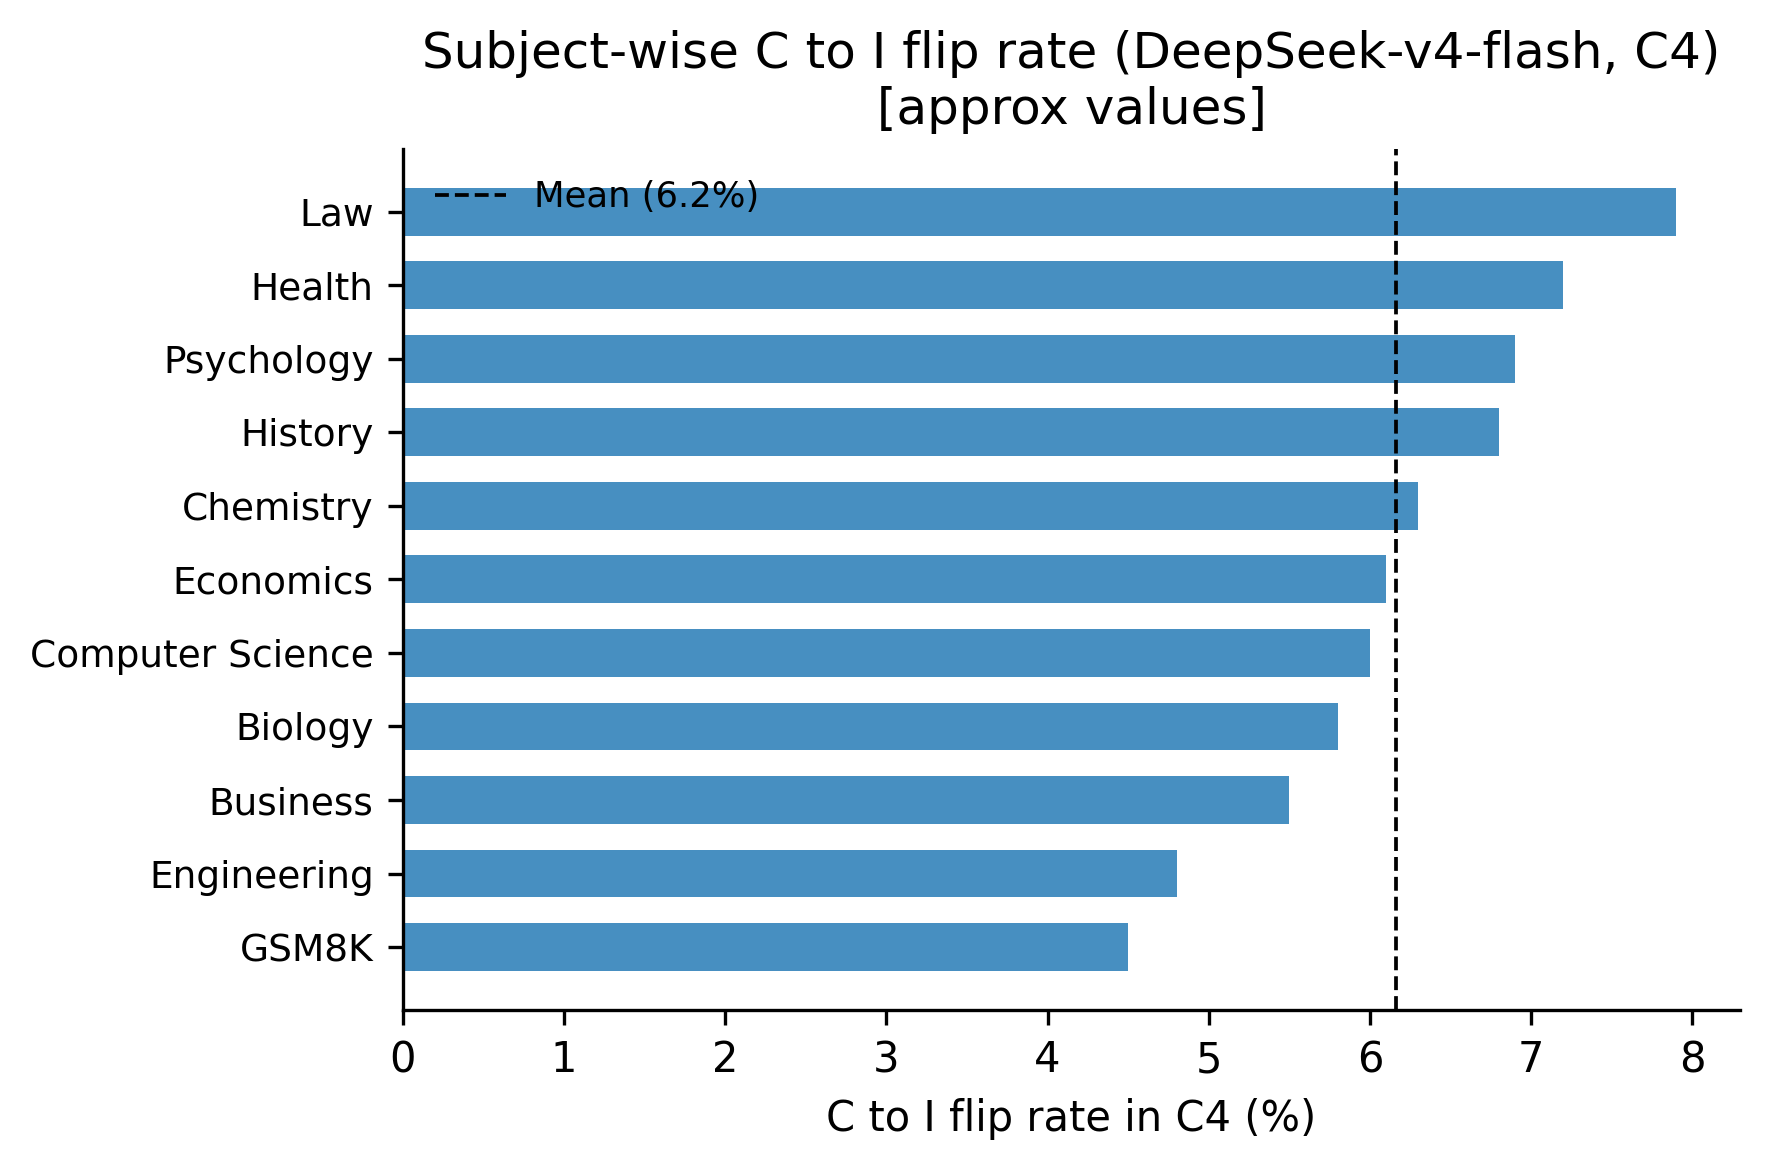
\includegraphics[width=0.72\linewidth]
    {images/figure3_subject_flip_rate.png}
  \caption{Correct-to-incorrect flip rate in C4 across MMLU-Pro subject
  categories and GSM8K, for \textit{DeepSeek-v4-flash}.
  Dashed vertical line: mean across subjects.
  Error bars: 95\% bootstrap CI.
  \label{sfig:subjects}}
\end{figure}

\bibliography{references}

\end{document}
